\subsection{Completamento e raffinamento delle funzionalità}
Questa fase comincia subito dopo la consegna dei documenti per la \textit{Revisione di Qualifica}, ovvero il 26-04-2021 e termina il 30-04-2021.\\
In questo periodo verranno creati ulteriori test per verificare il corretto funzionamento del prodotto. Se tutte le scadenze imposte dal gruppo vengono rispettate il tempo in eccesso viene occupato per la realizzazione di requisiti opzionali, concordati con il proponente. 

\subsubsection{Incremento VIII} 

\paragraph{Obiettivi}
\begin{itemize}
	\item Implementazione della gestione della sessione;
	\item Implementazione di un componente per l'esportazione dei parametri di configurazione dell'applicazione \textbf{[UC9]};
	\item Implementazione di un componente per l'importazione dei parametri di configurazione dell'applicazione \textbf{[UC1.2]}.
\end{itemize}
	
\paragraph{Periodi e attività} \mbox{}\\\mbox{}\\
Questo incremento si compone di un unico periodo, dal  26-04-2021 al 30-04-2021, con milestone fissata per l'ultimo giorno. Comprende attività di:	
\begin{itemize}
\item \textbf{Stesura:} incremento della documentazione da allegare al prodotto;
\item \textbf{Verifica dei documenti};
\item \textbf{Progettazione:} progettazione di un sistema per la gestione della sessione;
\item \textbf{Codifica:} codifica dei componenti per l'importazione e l'esportazione dei parametri di configurazione dell'applicazione;
\item \textbf{Verifica software:} verifica sulle funzionalità software aggiunte.
\end{itemize}

\begin{figure}[h]
	\centering
	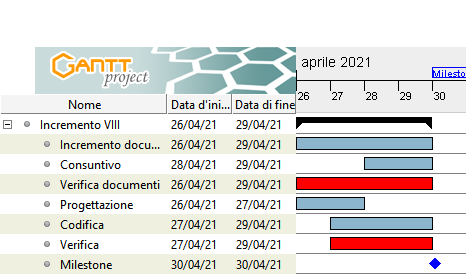
\includegraphics[width=12cm]{Images/GanttPianificazioneRaffinamentoFunzionalita.PNG}
	\caption{Diagramma di Gantt dell'attività di completamento e raffinamento delle funzionalità}
\end{figure}